%!TEX root = ../template.tex
%%%%%%%%%%%%%%%%%%%%%%%%%%%%%%%%%%%%%%%%%%%%%%%%%%%%%%%%%%%%%%%%%%%%
%% chapter3.tex
%% NOVA thesis document file
%%
%% Chapter with iCBD project
%%%%%%%%%%%%%%%%%%%%%%%%%%%%%%%%%%%%%%%%%%%%%%%%%%%%%%%%%%%%%%%%%%%%


%%-------------------------------------------------------------------
%%	3 - iCBD - Infrastructure for Client-Based (Virtual) Desktop (Computing)
%%-------------------------------------------------------------------
\chapter{iCBD - Infrastructure for Client-Based Desktop}
\label{cha:icbd}

The acronym iCBD stands for Infrastructure for Client-Based (Virtual) Desktop (Computing), a platform being developed by an R\&D partnership between\textit{ NOVA LINCS}, the Computer Science research unit hosted at the \textit{Departamento de Informática of Faculdade de Ciências e Tecnologia of Universidade NOVA de Lisboa} (DI - FCT NOVA) and \textit{SolidNetworks – Business Consulting, Lda}, a subsidiary of \textit{Reditus S.A.} group. 

iCBD’s primary goal is to implement a client-based VDI, a specialized form of \gls{VDI} where all computing chores – from graphical display to application execution – are performed directly on the user’s workstation (PC/laptop, etc.) hardware as opposed to performed on big and expensive servers, as it goes with mainstream VDI implementations such as the ones from Citrix, Microsoft or VMware, to name the most relevant ones. Furthermore, iCBD, while using the workstation’s hardware, does not touch the disk – either to load software or as a temporary scratch device: it runs diskless. And, however, it does offer a simple and centralised administration of the infrastructure, even when it spans multiple sites.

This chapter will address the project’s central concepts and associated technologies:

\begin{description}
	%
	\item [Section~\ref{sec:icbd_concept}] overviews the project’s core concepts and address note peculiarities and limitations of mainstream implementations in contrast with our approach.
	%
	\item [Section~\ref{sec:icbd_architecture}] studies the main architectural components of the platform, with emphasis on the different layers and how they act together to serve the end-user.
	%
\end{description}
\newpage


%%-------------------------------------------------------------------
%%	3.1 - The Concept
%%-------------------------------------------------------------------
\section{The Concept} % (fold)
\label{sec:icbd_concept}

iCBD, as a project, aims to research an architecture that leads to the development of a platform that we call client-based VDI, while maintaining all the benefits of both client-based and server-based VDI. Additionally, it should be deployable as a Cloud Desktop as a Service (DaaS) without any of the drawbacks of current DaaS offerings.

In short, our aim is to preserve the convenience and simplicity of a fully centralised management
platform for Linux and Windows desktops, instantiating those in the users' physical workstation from virtual machine templates (VMs) kept in repositories. We will further address this subject in Section~\ref{sec:icbd_architecture}.
\\
\\
To summarise the iCBD platform should be able to:

\begin{itemize}
	%
	\item Within the boundaries of the proposed architecture, adapt to a wide range of server configurations.
	%
	\item Provide an user experience so close to the traditional one, that users should not be able to tell it from a PC standard (local) install.
	%
	\item Simplify installation, maintenance and platform management tasks for the entire infrastructure, including servers in their multiple roles, storage and network devices, all from a single point of administration.
	%
	\item Allow for a highly competitive per-user/workstation cost.
	%
	\item Maintain an inter-site solution to support efficiently, e.g., a geographically disperse multi-site organisation.
	%
\end{itemize}


%%-------------------------------------------------------------------
%%	3.2 - The Architecture 
%%-------------------------------------------------------------------
\section{The Architecture} % (fold)
\label{sec:icbd_architecture}

%Topics:
%Introduce the layers
%Draw a diagram 
%Layers are a kind of role, not a single a defined service but a collection 

The iCBD platform encompasses the use of multiple services; to achieve a better understanding of its inner workings, we can group these services in four major architectural blocks, as seen in Figure~\ref{fig:icbd_layers}.


\begin{figure}[htbp]
	\centering
	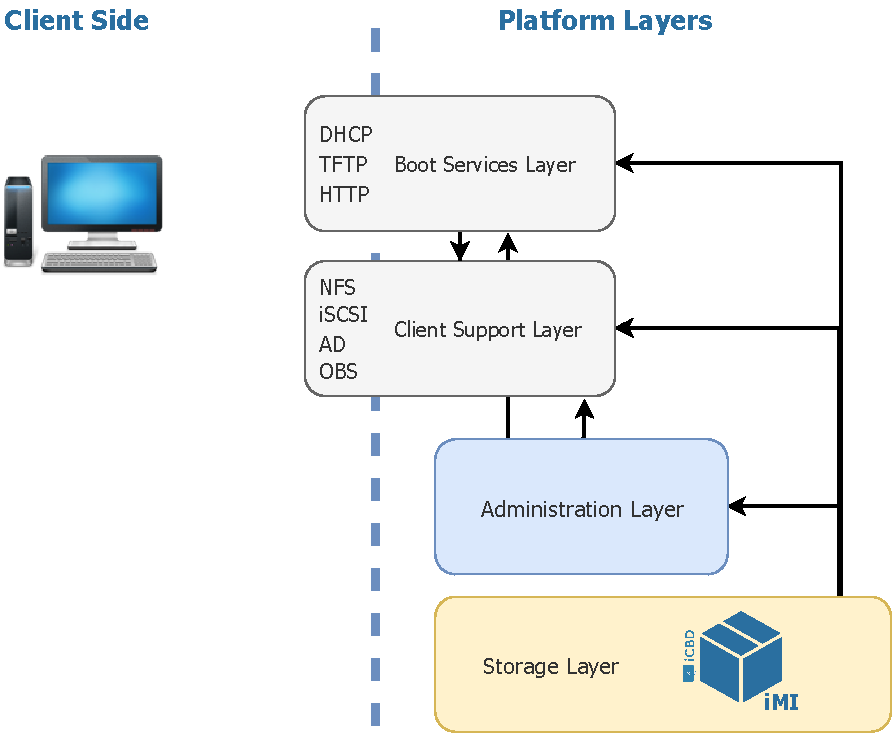
\includegraphics[height=4in]{cap3_iCBD_Layers}
	\caption{iCBD Layers View}
	\label{fig:icbd_layers}
\end{figure}


\begin{description}
	%
	\item [\acrfull{iMI}] embodies the required files to run a iCBD platform client; this nomenclature was borrowed and adapted from Amazon Web Services’ AMI~\cite{aws_ami}. An iMI includes a VM template (with an operating system, configurations and applications), the iCBD boot package (a collection of files needed for the network boot and tailored to the operating system) and an assortment of configurations for services like PXE and iSCSI.
	%
	\item [Boot Services Layer] responsible for providing the initial code that supports network boot of client machines, the transfer a bespoke follow-up package (OS, ramdrive, initial scripts), using services such as \acrshort{PXE}, \acrshort{DHCP}, \acrshort{TFTP} and \acrshort{HTTP}.
	%
	\item [Client Support Layer] provides support for client-side operations including, e.g., authentication, read/write storage space for client instances (since iMIs run on `diskless'' workstations) and access to the users' home directories.
	%deals with the demands of a deployed and running iCBD image, such as, providing read/write space (since iMIs run on diskless workstations) and storing users home directories. As well as, hosting domain controllers, centralised authentication amongst other services that can be already in place in the midst of a clients infrastructure. Granting the ability to deploy a customised iMI in any scenario.
	%
	\item [Administration Layer] maintains platform users and the full iMI life cycle, from creation to retirement. Currently, administration is based on a custom set of scripts.
	% takes advantage of a virtualisation stack (can be based in either \acrshort{KVM} or VMWare products) to engage in maintaining all the needed aspects for the successful creation and update processes of an \acrshort{iMI} lifecycle.  Employing a custom set of scripts, the creation of an iCBD Boot Package is also a duty of this layer. 
	%
	\item [Storage Layer] maintains the repository of iMIs and provides essential operations such as version control of the VM image files. Our work is fundamentally focused on this layer, extending it in such a way that a single repository abstraction can be built on top of the local/individual repositories through replication and caching. These local repositories are implemented on Btrfs or Ceph and may be exported to clients using \acrshort{NFS}, \acrshort{iSCSI}, REST and other suitable protocols.
	
	%Is also in this layer that we seize the potential of replication features provided by the file systems employed. In this project, the storage relies on two mainstream file systems: BTRFS and CEPH. Together with services like \acrshort{NFS} and \acrshort{iSCSI} enables a way to export data to clients.
\end{description}
 
In the next subsections, we will provide a more detailed description of each of the above-mentioned layers.

%%-------------------------------------------------------------------
%%	3.2. - iCBD Machine Image 
%%-------------------------------------------------------------------
\subsection{iCBD Machine Image}
\label{sub:icbd_imi}

\begin{figure}[htbp]
	\centering
	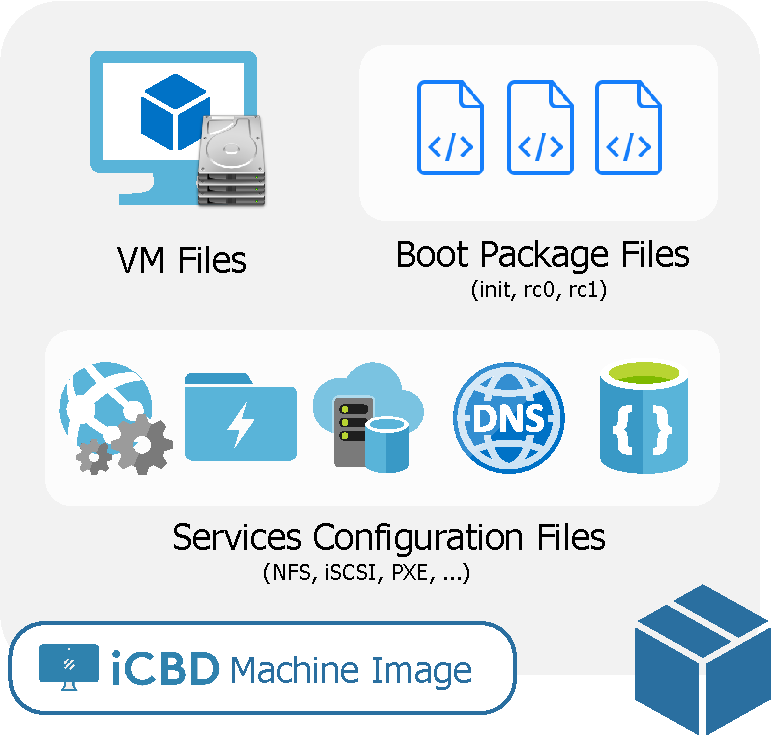
\includegraphics[height=4in]{cap3_iMI}
	\caption{iCBD Machine Image Files}
	\label{fig:icbd_iMI_files}
\end{figure}

In its essence, an iCBD Machine Image is an aggregation of everything that is needed to run an Operating System within the iCBD platform – kernel, binaries, data and configuration files. For the sake of simplicity, we categorise iMI files into three main groups:

\begin{description}
	%
	\item [VM Template files] The main component of this group is the virtual machine template in the form of a read-only image. As described in Section~\ref{sub:res_vm_storage}, the anatomy of a template follows the standard VMware and KVM formats either with multiple files (i.e., Virtual Disk Files like \texttt{.vmdk} or \texttt{.qcow}) or a \textit{raw} storage format (a disk image).
	%
	\item [iCBD Boot Package files] In a network boot environment, such as the one used, there is a need to keep a set of files that manage the boot process of the user’s workstation; these files can be included in the initial \textit{ramdisk} or transferred over HTTP later on, when needed. Included in the boot package are: a \textit{BusyBox} tool, an init file, and at least two Run Control Script files (\texttt{rc0} and \texttt{rc1}) that are responsible for starting network services, mount all file systems, and ultimately bring the system up into the single-user level. With \textit{BusyBox} (a single executable file with a stripped-down set of tools), a basic \textit{shell} is available during the boot process to fulfil all the required steps.
	%
	\item [Service Configuration files] The iCBD platform uses several services, and some do require particular settings in the configuration files. As an example, the `NFS exports'' configuration file should reflect which file systems are exported, which networks a remote host can use, as well as a myriad of options that NFS allows; the same happens to iSCSI, where an iSCSI target needs to refer to a backing store for the storage resource where the image resides. 
\end{description}

%\subsubsection{iMI Life Cycle}
\paragraph{iMI Life Cycle}
\label{subsub:icbd_imi_lifecycle}

The life cycle of an iMI encompasses all stages that take it throughout its course within the platform; Figure~\ref{fig:icbd_iMI_lifecycle} shows the major ones, from creation, through deployment, when in use by multiple clients and, finally, its retirement and placement in to temporary or cold storage.

\begin{figure}[htbp]
	\centering
	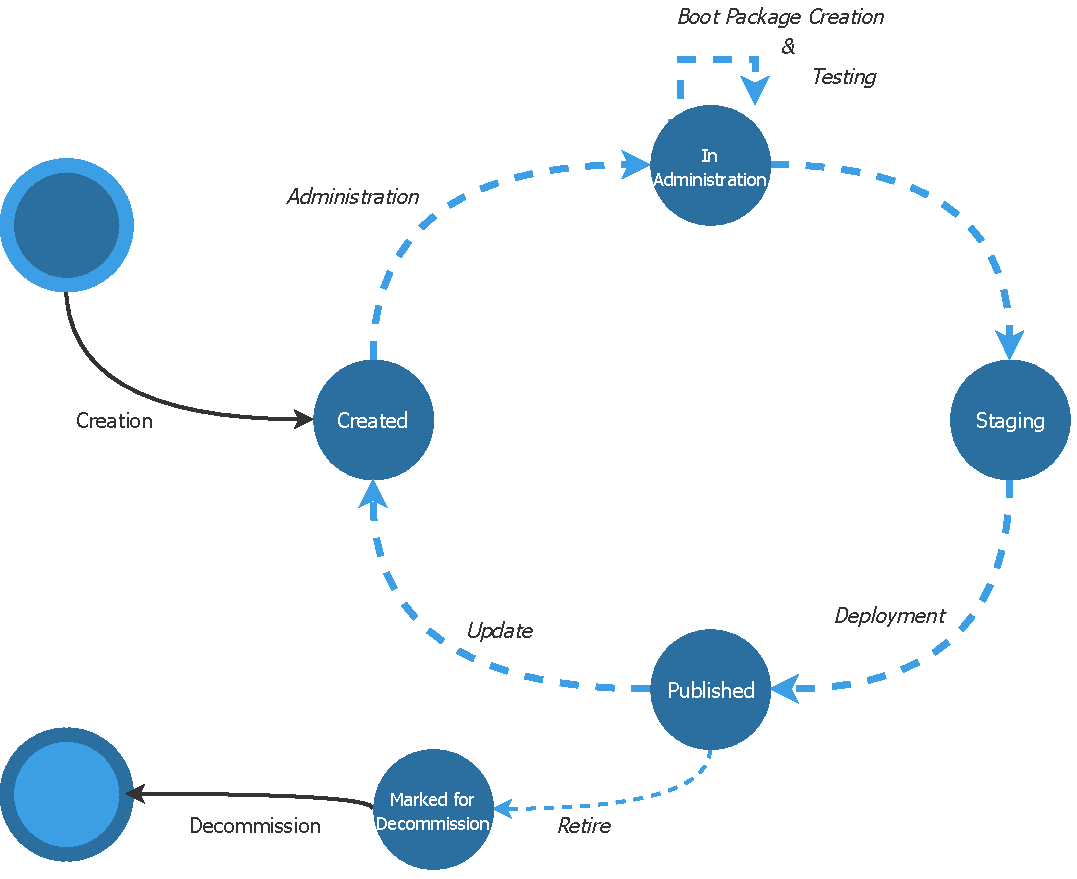
\includegraphics[height=4in]{cap3_iMI_Lifecycle}
	\caption{iMI Life Cycle inside the iCBD Platform}
	\label{fig:icbd_iMI_lifecycle}
\end{figure}

When an iMI completes a full cycle, a new version is created; so, every new update made to an iMI will spawn a new version. The creation of a new version is a rather straightforward and computationally light operation, thanks to the snapshotting features available at the storage layer.

During its life in the platform, an iMI can be in one of the following four main states:

\begin{description}
	\item [Created] After being inserted into the platform, an image is not instantaneously ready to be served to clients and booted in a workstation; it must pass through a number of administration steps for the generation of the appropriate boot package.
	%
	\item [In Administration] An iMI goes through this phase in two moments: the first one, described above, when an image has just been injected (created) into the platform; and the second, and most frequent case, when an image needs to be updated or, in any way, modified. The iMI will stay in this state as long as it is being managed, which can take from a few minutes to hours; at the end this process the boot package is automatically created.
	%
	\item [Not Published] This is the status of an image that is ready but isn’t yet published, and is therefore not visible to platform users. This phase is of particular interest for testing it for correctness of the boot process, and to ensure that the modifications were, in fact, applied. Only after testing should an iMI made available for general use.
	%
	\item [Published] This state corresponds to the deployment of an iMI into production and is the one where the iMI is expected to spend most of its time. iMIs in this stage have their entries displayed at the user’s workstation screen at boot time, and all the necessary support for their execution is available at the Boot Services Layer. So, if the user chooses one of those iMIs, no matter what device (e.g., PC or laptop) he/she is using, the image is expected to boot to completion, and the user should be able to login and work just as if the boot was from a local disk.
\end{description}

When an iMI completes a cycle and undergoes an update process, the old version is retired and set to a new state, named \textbf{Marked for Decommission}, which is comparable to a stay in limbo. First, because when the administration process was initiated clients could be using that same image, so it must be available for them (or else a disruption would happen). And, when the administration process finishes, 
clients may still be using the old version. Therefore, \textbf{Decommission} is only triggered when the last client “closes” its session. At that moment, the old version can be removed entirely from the platform or, more wisely, stored as a backup e.g., to allow the administrator to retrieve an older state of the image (for example, a newly installed update breaks some application).




%%-------------------------------------------------------------------
%%	3.2. - Boot Layer 
%%-------------------------------------------------------------------
\subsection{Boot Services Layer}
\label{sub:icbd_boot_layer}
% https://opensource.com/article/18/1/analyzing-linux-boot-process
% https://www.ibm.com/developerworks/library/l-linuxboot/index.html
% https://utcc.utoronto.ca/~cks/space/blog/linux/LinuxBootOverview?

%From an end-user perspective, the only layer that is visible and, for “power-users”, requires interaction, is the boot layer – one that displays the set of images the user is allowed to boot, and waits for his/her choice. However not every single aspect is noticeable: while this happens in the workstation’s screen, in the background multiple services cooperate to run the chosen iCBD Machine Image.

From an end-user perspective, the only layer that is visible and requires interaction, is the boot layer – one that displays the set of images the user is allowed to boot, and waits for his/her choice. However not every single aspect is noticeable: while this happens in the workstation’s screen, in the background multiple services cooperate to run the chosen iCBD Machine Image.

The iCBD platform provides two distinct ways to remote boot an iMI: one instantiates, from an iMI, a native Operating System that runs on the workstation’s “bare metal” just like a standard diskless network boot of, say, Linux does; the other uses the above mechanism to start a minimal OS with an embedded hypervisor installed, then runs the hypervisor, and finally launches another iMI, one chosen from those available in the platform. Both approaches are entirely transparent to the user and, users who are not knowledgeable about virtualisation technologies will be completely unaware of whether they are running a native or virtualised OS.

The first part of the boot process runs like any other network boot: a series of DHCP requests are used to provide suitable network parameters - particularly the location (IP address) of the TFTP server and, then, a small network boot manager program, is transferred, loaded and executed. Using the standard PXE boot environment, a friendly looking, tailored graphical menu, displays an assortment of choices that announces the different iMIs ready to boot.

%\subsubsection{Booting an iMI in a Workstation }
\paragraph{Booting an iMI in a Workstation}
\label{subsub:icbd_booting_imi}

After the selection, in the PXE~\cite{ibm_linux_boot} boot menu, of one of the available iMIs , the second-stage boot kicks in, using \textit{PXELINUX} as a bootloader. That provides us with the capability of transferring a compressed Linux Kernel (\texttt{vmlinuz}) and an initial ramdisk (\texttt{initramfs})~\cite{ibm_initrd} using either TFTP or HTTP. In this step, a number of parameters needed for proper operation are set with their appropriate values based on the requirements of the chosen image. After loading everything into memory (RAM), the second-stage bootloader runs the kernel image which, after initialisation, starts the first user-space application – usually, the init program.

In the iCBD platform init starts a chain of execution of two custom files, \texttt{rc0} and \texttt{rc1}; these Run Control scripts configure every single aspect in the OS according to the hardware characteristics of physical machine that is booting. The first step is to reconfigure the network interface card and obtain IP connectivity. Then, a check is performed to see if there is a need of getting more files to complete the boot process and, if necessary, those files are transferred. The next script, deals with data volumes and mounting operations – R/W space, user home directories, etc.. If the image’s OS is just the platform to run another iMI in virtualisation mode, more configuration steps are performed, e.g., a check is made to determine if the base OS file system happens to be Btrfs: if true, seeding must be used in order to create a R/W instance from an R/O iMI. Alternatively, or if the iMI OS is not Btrfs, an overlay filesystem is used to create the R/W instance.

After these configuration steps, the \texttt{switch root} command is executed moving the (already mounted) filesystems \texttt{/proc}, \texttt{/dev}, \texttt{/sys}, \texttt{/tmp} and \texttt{/run} to a new root and turning it into the new root filesystem, performing some housekeeping, namely erasing all files not in use in the \texttt{initramfs} root, releasing any unused memory.

Finally, the remaining configuration steps include setting of the current time with the NTP service and logging some statistics such as the elapsed time and the bandwidth consumed by the boot process as a whole.



%%-------------------------------------------------------------------
%%	3.2. - Administration Layer 
%%-------------------------------------------------------------------
\subsection{Administration Layer}
\label{sub:icbd_adm_layer}

One of the most important features provided by the platform is the ability to perform administration operations on an iMI, a task accomplished with the help of an administration tool which enables an iCBD administrator (or architect, if we draw a parallel with a role commonly found in private cloud infrastructures) in an organisation to make the changes he/she deems necessary (e.g., update the OS and applications, add or remove software, and modify configurations) and then publish the new image (version) for widespread use.



%\subsubsection{The Administration Process}
%\label{subsub:admin_imi}

%\textbf{The Administration Process}
\paragraph{The Administration Process}
\label{par:admin_imi}

The administration tool consists of a main script, \texttt{adm}, which then calls a series of others, depending on the task at hand. Calling \texttt{adm} with the name of one iMI as an argument starts an administration appliance - a VM with a custom-tailored base image that will support the administration process. Usually, the VM guest OS will be Linux, with several distributions supported: openSUSE Leap 42.2, Fedora 27, CentOS 7 and Ubuntu 16.04 LTS. The whole administration process makes extensive use of the snapshotting capabilities of the Storage Layer (whether using Btrfs or Ceph), with no (predictable) performance degradation on the other iCBD platform services.

For each iMI, there is a snapshot with an index number that relates to its version and age (i.e., higher numbers represent more recent versions); that index is used as the name of a directory, and the snapshot (and related files) are kept inside that directory. So, creating a new linked clone from the latest version of a VM becomes a very simple process.

When booted, the administration VM will start a hypervisor (VMware Workstation, VMware Player
or KVM) and the hypervisor will be instructed to boot a linked clone created on-the-fly from the VM version (i.e., the iMI) that the administrator wishes to update. Thus, this process will, if executed in the iCBD administration server itself, use nested virtualisation~\cite{kvm_nested} to achieve its goal, which may result in some performance degradation (even considering the use of a Type 1 hypervisor, such as KVM). However, in theory, nothing prevents the administrator from using his/her workstation in native mode or a server with a bare-metal hypervisor and run the administration VM using only one level of virtualisation.

In this step, the (newly created) snapshot being managed is in a temporary directory, one whose lifetime is the duration of the procedure. This method serves two purposes: first, all clients using the iMI version that is undergoing changes can keep using it; and, last, one may quickly discard all changes made in the working directory version if one wishes so.

When all modifications have been made to the temporary image, the administrator is given the option whether to commit or discarding them; if one commits, the temporary (working) directory is used to create a new linked clone (of the temporary snapshot), but one that follows the naming rules, and may, therefore, be used as the name of the new directory.


%\subsubsection{Creating the boot package}
%\label{subsub:createboot_imi}

\paragraph{Creating the boot package}
\label{par:icbd_create_bootpack}

After completion of the above-described steps, the iMI is not yet ready to be published, as there are no files to support the boot process; the next step is, therefore, the creation of a boot package. This is the responsibility of the \texttt{mki} script, one that, depending on the type of the iMI, may be called immediately when the Administration Process is over by the \texttt{adm} tool.

The procedure is different for Windows or Linux iMIs: while sharing a common set of steps, Linux iMIs require an additional number of customisation steps because iMIs for Linux have two sub-types – one for iMIs intended to run natively on a workstation, and the other for iMIs that serve as hosts for other images. The first type requires the creation of custom \texttt{initramfs} and \texttt{vmlinuz} files, the addition of a subset of the image's Kernel drivers and firmware (namely for all available network interfaces and the filesystems used during the boot process), and the customisation of Run Control scripts (\texttt{rc0} and \texttt{rc1}) that start the network services with a suitable configuration, compatible with the iCBD platform, and mount the correct remote file systems. At the end of this process, a script called \texttt{runvm} is also added; that script is instrumental in starting a virtualised iMI, as well as in configuring the hypervisor parameters in order to take advantage of the client’s hardware.

However, the job of the \texttt{mki} script is not yet complete: for the two types of iMIs, the configuration of both the \textit{iSCSI targets} (to reflect the new iMI version) and the \textit{pxelinux} (to reflect the new paths to the files that will be served to the clients) must be updated.


%%-------------------------------------------------------------------
%%	3.2. - Client Layer 
%%-------------------------------------------------------------------
\subsection{Client Support Layer}
\label{sub:icbd_client_support_layer}

The Client Support Layer is the most fluid of all layers, containing an aggregation of services (most of them originated outside the platform) working together to provide the environment that is required for a client workstation to operate correctly. Another essential service provided by this layer is its relation with storage layer, one which, using protocols such as NFS and iSCSI, allows the client to provide the necessary data for the boot process and obtain read/write space to support the changes made to the client’s storage instance (derived from the iMI). Moreover, these protocols are the ones that provide access to the user home directory and other volumes, if supported.

It is important to note that there are other services that are essential to the correct operation of clients in the iCBD platform, such as DNS and NTP. And there are also services that, while not directly related to the iCBD platform, are nevertheless need to support clients; as an example, in a medium/large organisation Microsoft’s Active Directory plays a paramount role – therefore it is necessary for the iCBD platform to coexist with this type of service, and Windows iMIs can be prepared in a way that, when an instance is booted, it will “automatically” join the organisation’s AD.

%!!! \textbf{TODO} !!!

%\textbf{TOPICS :}
%\begin{itemize}
%	\item Provide r/w space (for the duration of the session)
%	\item Stores users directories (Home directory)
%	\item Keep core services like DHCP, NTP, DNS, ...
%	\item Integrate with external services such as Samba shares, LDAP, Active directory, ..
%\end{itemize}


%%-------------------------------------------------------------------
%%	3.2. - Storage Layer 
%%-------------------------------------------------------------------
\subsection{Storage Layer}
\label{sub:icbd_storage_layer}

The most significant part of our work will focus on this layer, which is responsible for storing all platform data, whether they are iMIs, virtual disks (\texttt{.vmdk}) for VMs such as the administration VM and others that support platform services, databases that preserve information and configuration data for those services, code repositories, etc.. In its essence, the Storage layer consists of a set of file systems (or, if OBS-based, of object stores) each with its own purpose.

To keep this document short, we will only focus on file systems that provide storage for iMIs. Given the uniqueness of this type of data, the file system must have the right set of features, and of particular importance is the support for snapshots; as we have previously referred, our choice is Btrfs. It is important to mention that this is not the only solution that supports snapshots – object stores such as RADOS (from Ceph) are particularly well suited to store very large objects, such as virtual disks, but that avenue is being researched in another project. 

The Btrfs features that are heavily used in the iCBD platform are: sub-volumes; snapshots; cloning of both sub-volumes and snapshots; Btrfs seeding; and incremental backups, just to name a few. These features are used achieve several goals: multiple sub-volumes are used to store different parts of the platform data, snapshots are widely used to create (a kind of) version control for iMIs (allowing us to access any version at any moment) and to backup the entire iCBD platform. Btrfs seeding is another important feature, as it provides a mechanism that allows multiple read-only mounts of the same Btrfs file system, thus enabling multiple clients to use the same iMI.

One must remember that, while this work is focused on Btrfs, from the point of view of the remaining
layers the type of store - filesystem or object-based - should be entirely transparent to the other layers, which will interface iCBD “data objects” through standard, widespread protocols such as NFS or iSCSI. 

Therefore, when dealing with the problem of data replication across multiple file systems transparency, as an attribute, is fundamental. We will discuss in detail the replication and caching topics in the next chapter, and we will provide, then, an explanation of the decision-making process and a discussion on the implementation issues.



%!!! \textbf{TODO} !!!

%\textbf{TOPICS :}
%\begin{itemize}
%	\item Why btrfs? (Snapshots, seeding)
%	\item How are files stored?
%	\item The use of BTRFS multiple subvolumes for different parts of the platform.
%	\item The use of cloning to save multiple versions of an iMI, giving the possibility to roll back unwanted changes.
%	\item The need to replicate data - multiple locations and cache server (one of the focus of the thesis)
%	\item Should be transparent the the remaining layers. As being develop in Joao's thesis the use of CEPH  should be used with little to none modifications to other layers. (Interfacing through NFS or iSCSI just like BTRFS)
%\end{itemize}

%https://blogs.oracle.com/developers/save-disk-space-on-linux-by-cloning-files-on-btrfs-and-ocfs2-v2
%In this case the file system does not create a new link pointing to an existing inode, it rather creates a new inode that shares the same disk blocks as the original file. This means that this operation only works within the boundaries of the same file system or subvolume. The outcome looks very much like a copy of the source file, but the actual data blocks have not been duplicated. Due to the copy-on-write nature, a modification of any one of the files will not be visible in the other file. Note that this should not be confused with hard links – this web page provides a good explanation of the differences.

%For Btrfs, you can invoke this feature by using the cp(1) utility with the --reflink option, which was added to the GNU coreutils in version 7.5 (released in Aug. 2009):


%For each iMI, there is a snapshot with an index number that relates to its version and age (the higher the number the most recent the version is).
%Multiple versions of an iMI are stored in directories named by the index of the version. So, is simple to create a new linked clone from the most recent version 

%\textbf{TODO - Talk about btrfs seed}
%The importance of btrfs seeding relays on the fact that this feature alows for the multiple mounting operation of the same file system in read only mode. Thus allowing multiple clients to use the same image.. (Fulcral to the the platform)
%http://www.oracle.com/technetwork/articles/servers-storage-admin/advanced-btrfs-1734952.html 


